\documentclass[tikz,border=3pt]{standalone}
\usepackage{amsmath,amssymb}
\usetikzlibrary{arrows.meta,calc,decorations.pathreplacing,positioning}

\newcommand{\Enc}{E_\theta}
\newcommand{\Dec}{D_\phi}

\definecolor{basinblue}{HTML}{2F6DB3}
\definecolor{basingreen}{HTML}{4B9B3B}
\definecolor{basinorange}{HTML}{E7832C}
\definecolor{ink}{HTML}{20242A}
\definecolor{softgray}{HTML}{EEF1F5}
\definecolor{midgray}{HTML}{808895}
\definecolor{panelgray}{HTML}{F7F8FA}

\newcommand{\drawmask}[4]{%
  \foreach \i/\v in {#4}{%
    \pgfmathsetmacro{\xx}{#1+\i*0.205}%
    \ifnum\v=1
      \fill[#3!34] (\xx,#2) rectangle ++(0.18,0.18);
      \draw[#3!70!black,line width=0.25pt] (\xx,#2) rectangle ++(0.18,0.18);
    \else
      \fill[white] (\xx,#2) rectangle ++(0.18,0.18);
      \draw[midgray!45,line width=0.22pt] (\xx,#2) rectangle ++(0.18,0.18);
    \fi
  }%
}

\newcommand{\drawtinymask}[4]{%
  \foreach \i/\v in {#4}{%
    \pgfmathsetmacro{\xx}{#1+\i*0.155}%
    \ifnum\v=1
      \fill[#3!45] (\xx,#2) rectangle ++(0.13,0.13);
      \draw[#3!75!black,line width=0.18pt] (\xx,#2) rectangle ++(0.13,0.13);
    \else
      \fill[white] (\xx,#2) rectangle ++(0.13,0.13);
      \draw[midgray!40,line width=0.16pt] (\xx,#2) rectangle ++(0.13,0.13);
    \fi
  }%
}

\begin{document}
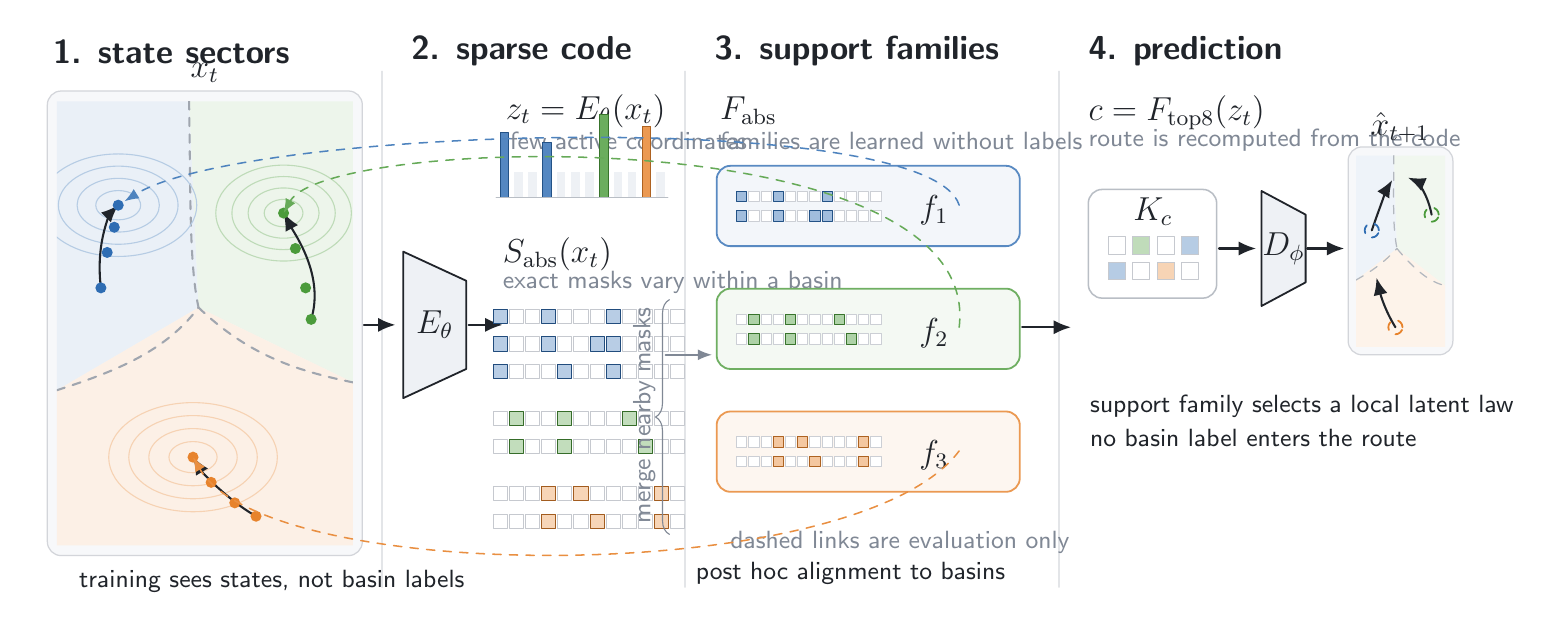
\begin{tikzpicture}[
  x=1cm,y=1cm,
  font=\sffamily,
  >=Latex,
  line cap=round,
  line join=round,
  arrow/.style={-{Latex[length=2.2mm,width=1.8mm]},line width=0.75pt,draw=ink},
  softarrow/.style={-{Latex[length=1.8mm,width=1.4mm]},line width=0.55pt,draw=midgray},
  panel/.style={rounded corners=5pt,draw=midgray!35,fill=panelgray,line width=0.45pt},
  title/.style={font=\sffamily\bfseries\large,text=ink},
  label/.style={font=\sffamily\small,text=ink},
  mathlabel/.style={font=\sffamily\large,text=ink},
  note/.style={font=\sffamily\small,text=midgray}
]

% Figure sectors.
\fill[white] (-0.05,-0.05) rectangle (18.25,7.35);
\node[title,anchor=west] at (0.15,7.05) {1. state sectors};
\node[title,anchor=west] at (4.70,7.05) {2. sparse code};
\node[title,anchor=west] at (8.55,7.05) {3. support families};
\node[title,anchor=west] at (13.30,7.05) {4. prediction};

\draw[midgray!22,line width=0.55pt] (4.45,0.25) -- (4.45,6.80);
\draw[midgray!22,line width=0.55pt] (8.30,0.25) -- (8.30,6.80);
\draw[midgray!22,line width=0.55pt] (13.05,0.25) -- (13.05,6.80);

% 1. State-space basin sectors.
\draw[panel] (0.20,0.65) rectangle (4.20,6.55);
\begin{scope}
  \clip (0.32,0.78) rectangle (4.08,6.42);
  \coordinate (junction) at (2.12,3.80);
  \fill[basinblue!10] (0.32,6.42) -- (2.00,6.42) -- (junction) -- (0.32,2.75) -- cycle;
  \fill[basingreen!10] (2.00,6.42) -- (4.08,6.42) -- (4.08,2.85) -- (junction) -- cycle;
  \fill[basinorange!12] (0.32,0.78) -- (4.08,0.78) -- (4.08,2.85) -- (junction) -- (0.32,2.75) -- cycle;

  \draw[midgray!75,dashed,line width=0.75pt] (2.00,6.42) .. controls (2.02,5.25) and (2.00,4.35) .. (junction);
  \draw[midgray!75,dashed,line width=0.75pt] (0.32,2.75) .. controls (1.10,3.00) and (1.70,3.25) .. (junction);
  \draw[midgray!75,dashed,line width=0.75pt] (junction) .. controls (2.75,3.20) and (3.35,3.00) .. (4.08,2.85);

  \foreach \r in {0.30,0.55,0.80,1.05} {
    \draw[basinblue!35,line width=0.4pt] (1.10,5.10) ellipse ({0.95*\r} and {0.62*\r});
    \draw[basingreen!36,line width=0.4pt] (3.20,5.00) ellipse ({0.82*\r} and {0.58*\r});
    \draw[basinorange!36,line width=0.4pt] (2.05,1.90) ellipse ({1.02*\r} and {0.66*\r});
  }

  \draw[basinblue,arrow] (0.88,4.05) .. controls (0.80,4.70) and (1.05,5.05) .. (1.10,5.10);
  \draw[basingreen,arrow] (3.55,3.65) .. controls (3.72,4.20) and (3.35,4.72) .. (3.20,5.00);
  \draw[basinorange,arrow] (2.85,1.15) .. controls (2.50,1.35) and (2.17,1.70) .. (2.05,1.90);
  \foreach \p in {(0.88,4.05),(0.96,4.50),(1.05,4.82),(1.10,5.10)}{\fill[basinblue] \p circle (2.0pt);}
  \foreach \p in {(3.55,3.65),(3.48,4.05),(3.35,4.55),(3.20,5.00)}{\fill[basingreen] \p circle (2.0pt);}
  \foreach \p in {(2.85,1.15),(2.58,1.32),(2.28,1.58),(2.05,1.90)}{\fill[basinorange] \p circle (2.0pt);}
\end{scope}
\node[mathlabel] at (2.20,6.78) {$x_t$};
\node[label,anchor=west] at (0.48,0.32) {training sees states, not basin labels};

% State samples and encoder.
\draw[arrow] (4.22,3.58) -- (4.62,3.58);
\draw[fill=softgray,draw=ink,line width=0.65pt] (4.72,2.65) -- (5.52,3.02) -- (5.52,4.14) -- (4.72,4.51) -- cycle;
\node[mathlabel] at (5.12,3.58) {$\Enc$};

% 2. Sparse latent code and exact supports.
\draw[arrow] (5.55,3.58) -- (5.98,3.58);
\node[mathlabel,anchor=west] at (5.90,6.30) {$z_t=\Enc(x_t)$};
\node[note,anchor=west] at (5.95,5.92) {few active coordinates};
\foreach \i in {0,...,11}{
  \pgfmathsetmacro{\xx}{5.95+\i*0.18}
  \fill[softgray] (\xx,5.20) rectangle ++(0.11,0.32);
}
\foreach \i/\h/\col in {0/0.82/basinblue,3/0.70/basinblue,7/1.05/basingreen,10/0.90/basinorange}{
  \pgfmathsetmacro{\xx}{5.95+\i*0.18}
  \fill[\col!82] (\xx,5.20) rectangle ++(0.11,\h);
  \draw[\col!75!black,line width=0.25pt] (\xx,5.20) rectangle ++(0.11,\h);
}
\draw[midgray!55,line width=0.35pt] (5.90,5.20) -- (8.08,5.20);

\node[mathlabel,anchor=west] at (5.86,4.48) {$S_{\rm abs}(x_t)$};
\node[note,anchor=west] at (5.86,4.12) {exact masks vary within a basin};
\drawmask{5.86}{3.60}{basinblue}{0/1,1/0,2/0,3/1,4/0,5/0,6/0,7/1,8/0,9/0,10/0,11/0}
\drawmask{5.86}{3.25}{basinblue}{0/1,1/0,2/0,3/1,4/0,5/0,6/1,7/1,8/0,9/0,10/0,11/0}
\drawmask{5.86}{2.90}{basinblue}{0/1,1/0,2/0,3/0,4/1,5/0,6/0,7/1,8/0,9/0,10/0,11/0}
\drawmask{5.86}{2.30}{basingreen}{0/0,1/1,2/0,3/0,4/1,5/0,6/0,7/0,8/1,9/0,10/0,11/0}
\drawmask{5.86}{1.95}{basingreen}{0/0,1/1,2/0,3/0,4/1,5/0,6/0,7/0,8/0,9/1,10/0,11/0}
\drawmask{5.86}{1.35}{basinorange}{0/0,1/0,2/0,3/1,4/0,5/1,6/0,7/0,8/0,9/0,10/1,11/0}
\drawmask{5.86}{1.00}{basinorange}{0/0,1/0,2/0,3/1,4/0,5/0,6/1,7/0,8/0,9/0,10/1,11/0}

% 3. Support families.
\draw[softarrow] (8.05,3.20) -- (8.64,3.20);
\draw[decorate,decoration={brace,amplitude=5pt},draw=midgray] (8.10,0.92) -- (8.10,3.90);
\node[note,rotate=90] at (7.78,2.43) {merge nearby masks};

\node[mathlabel,anchor=west] at (8.62,6.30) {$F_{\rm abs}$};
\node[note,anchor=west] at (8.62,5.92) {families are learned without labels};

\draw[rounded corners=5pt,draw=basinblue!80,fill=basinblue!6,line width=0.65pt] (8.70,4.58) rectangle (12.55,5.60);
\drawtinymask{8.95}{5.15}{basinblue}{0/1,1/0,2/0,3/1,4/0,5/0,6/0,7/1,8/0,9/0,10/0,11/0}
\drawtinymask{8.95}{4.90}{basinblue}{0/1,1/0,2/0,3/1,4/0,5/0,6/1,7/1,8/0,9/0,10/0,11/0}
\node[mathlabel,anchor=west] at (11.15,5.04) {$f_1$};

\draw[rounded corners=5pt,draw=basingreen!80,fill=basingreen!6,line width=0.65pt] (8.70,3.02) rectangle (12.55,4.04);
\drawtinymask{8.95}{3.59}{basingreen}{0/0,1/1,2/0,3/0,4/1,5/0,6/0,7/0,8/1,9/0,10/0,11/0}
\drawtinymask{8.95}{3.34}{basingreen}{0/0,1/1,2/0,3/0,4/1,5/0,6/0,7/0,8/0,9/1,10/0,11/0}
\node[mathlabel,anchor=west] at (11.15,3.48) {$f_2$};

\draw[rounded corners=5pt,draw=basinorange!82,fill=basinorange!7,line width=0.65pt] (8.70,1.46) rectangle (12.55,2.48);
\drawtinymask{8.95}{2.03}{basinorange}{0/0,1/0,2/0,3/1,4/0,5/1,6/0,7/0,8/0,9/0,10/1,11/0}
\drawtinymask{8.95}{1.78}{basinorange}{0/0,1/0,2/0,3/1,4/0,5/0,6/1,7/0,8/0,9/0,10/1,11/0}
\node[mathlabel,anchor=west] at (11.15,1.92) {$f_3$};

\node[note,anchor=west] at (8.75,0.82) {dashed links are evaluation only};
\draw[softarrow,dashed,draw=basinblue!85] (11.78,5.10) .. controls (11.40,6.35) and (2.70,6.10) .. (1.18,5.15);
\draw[softarrow,dashed,draw=basingreen!85] (11.78,3.55) .. controls (12.10,6.20) and (3.75,6.00) .. (3.20,5.00);
\draw[softarrow,dashed,draw=basinorange!90] (11.78,1.98) .. controls (10.50,0.25) and (3.00,0.25) .. (2.05,1.90);
\node[label,fill=white,inner sep=1.5pt] at (10.40,0.42) {post hoc alignment to basins};

% 4. Prediction route.
\draw[arrow] (12.58,3.55) -- (13.20,3.55);
\node[mathlabel,anchor=west] at (13.30,6.28) {$c=F_{\rm top8}(z_t)$};
\node[note,anchor=west] at (13.30,5.92) {route is recomputed from the code};

\draw[rounded corners=5pt,draw=midgray!55,fill=white,line width=0.55pt] (13.42,3.92) rectangle (15.05,5.30);
\node[mathlabel] at (14.24,5.02) {$K_c$};
\foreach \x/\y/\c in {13.67/4.16/basinblue,13.98/4.48/basingreen,14.29/4.16/basinorange,14.60/4.48/basinblue}{
  \fill[\c!35] (\x,\y) rectangle ++(0.22,0.22);
  \draw[midgray!50,line width=0.2pt] (\x,\y) rectangle ++(0.22,0.22);
}
\foreach \x in {13.67,13.98,14.29,14.60}{
  \foreach \y in {4.16,4.48}{
    \draw[midgray!45,line width=0.18pt] (\x,\y) rectangle ++(0.22,0.22);
  }
}

\draw[arrow] (15.08,4.55) -- (15.55,4.55);
\draw[fill=softgray,draw=ink,line width=0.65pt] (15.62,3.82) -- (16.18,4.12) -- (16.18,4.98) -- (15.62,5.28) -- cycle;
\node[mathlabel] at (15.90,4.55) {$\Dec$};
\draw[arrow] (16.20,4.55) -- (16.67,4.55);

\draw[panel] (16.72,3.20) rectangle (18.05,5.84);
\node[mathlabel] at (17.38,6.08) {$\hat{x}_{t+1}$};
\begin{scope}
  \clip (16.82,3.30) rectangle (17.95,5.73);
  \fill[basinblue!8] (16.82,5.73) -- (17.30,5.73) -- (17.34,4.55) -- (16.82,4.15) -- cycle;
  \fill[basingreen!8] (17.30,5.73) -- (17.95,5.73) -- (17.95,4.08) -- (17.34,4.55) -- cycle;
  \fill[basinorange!10] (16.82,3.30) -- (17.95,3.30) -- (17.95,4.08) -- (17.34,4.55) -- (16.82,4.15) -- cycle;
  \draw[midgray!60,dashed,line width=0.45pt] (17.30,5.73) .. controls (17.30,5.20) and (17.28,4.85) .. (17.34,4.55);
  \draw[midgray!60,dashed,line width=0.45pt] (16.82,4.15) .. controls (17.05,4.28) and (17.18,4.38) .. (17.34,4.55);
  \draw[midgray!60,dashed,line width=0.45pt] (17.34,4.55) .. controls (17.56,4.28) and (17.76,4.12) .. (17.95,4.08);
  \draw[basinblue,arrow] (17.02,4.78) .. controls (17.13,5.10) and (17.22,5.32) .. (17.28,5.42);
  \draw[basingreen,arrow] (17.78,4.98) .. controls (17.72,5.30) and (17.55,5.42) .. (17.48,5.45);
  \draw[basinorange,arrow] (17.32,3.55) .. controls (17.18,3.78) and (17.13,3.97) .. (17.08,4.18);
  \draw[basinblue,dashed,line width=0.65pt] (17.02,4.78) circle (0.09);
  \draw[basingreen,dashed,line width=0.65pt] (17.78,4.98) circle (0.09);
  \draw[basinorange,dashed,line width=0.65pt] (17.32,3.55) circle (0.09);
\end{scope}

\node[label,anchor=west] at (13.32,2.55) {support family selects a local latent law};
\node[label,anchor=west] at (13.32,2.15) {no basin label enters the route};

\end{tikzpicture}
\end{document}
